\subsection{Session Management}

MicroNet provides session management as a high level feature to tackle the
integral part of session handling in a \og{}. Player sessions are essential to
track actions of individual players and persist the progress of a player. Game
sessions tackle the issue that \ogs{} are state-full and therefore game session
in simulation services are unique. 

Session management has been one major issue throughout thesis one, two and
three. The final solution for session management relies on a NoSQL database.




\subsubsection{Player Sessions}

The authentication process that has briefly been mentioned in
\autoref{sub:networking} is responsible to establish player sessions. Once
authenticated player sessions can be used to collate incoming messages to users.
Player sessions can also be used to store frequently changing player data to
allow fast and global access. In MicroNet the player sessions can be accessed
through Couchbase.

One drawback that player session introduce is the fact that multiple API
gateways each gateway needs the ability to look-up player connections to
determine if the corresponding user is authenticated. This process has to be
done upon every player message which leads a lot of access to NoSQL. Another
possibility would be that the user needs to send a authentication cookie with
every message. This method introduces significant bandwidth overhead which is
worse. 

\begin{figure}
	\centering
  	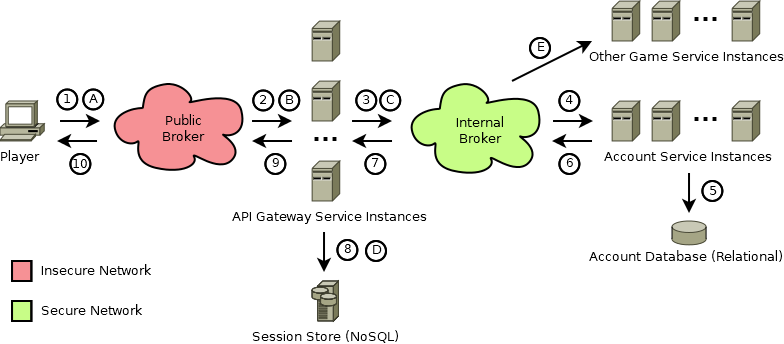
\includegraphics[width=\textwidth]{images/architecture/PlayerSessions}
	\caption{Player session authentication process.}
	\label{fig:player_sessions}
\end{figure}

\autoref{fig:player_sessions} shows the whole authentication process with the
result of a established authenticated player connection. The message flow
consists of the following steps:

\begin{enumerate}
  \item The user sends a login request to the public broker.
  \item One API Gateway polls the message in a competing consumer fashion.
  \item The gateway forwards the login message to the internal broker using the
  mn://account/login queue.
  \item One Account Service polls the message in a competing consumer fashion.
  \item The Account Service authenticates the user using the Account Database.
  \item The account service returns the login response to a temporary queue held
  open by the responsible gateway.
  \item The gateway service consumes the login response from the temporary
  queue.
  \item Upon login success the gateway adds a new player session to the session
  store, identified by the player connection.
  \item The gateway returns the login response to a temporary queue held open by
  the requesting player.
  \item The player consumes the login response from a temporary queue. Upon
  success he gains access to the game services (A, B, C, D\footnote{In step D
  the API Gateway must verify if the player connection is already
  authenticated. If the player is not authenticated no messages are forwarded.},
  E).
\end{enumerate}



\subsubsection{Game Sessions}

Game sessions are a strategy to deal with the state-fullness of \ogs{}. Game
sessions are unique and a player can only be in one game session at a time. Game
sessions are either infinitely or terminate at specific conditions. Either way
the player must be able to find the correct simulation instance which hosts the
game session he wants to participate in. MicroNet provides this functionality
through the WorldService which is part of the service catalogue.

\begin{figure}
	\centering
  	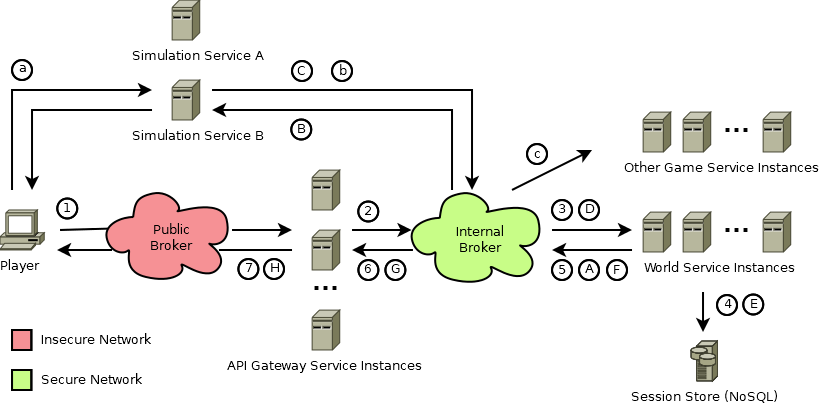
\includegraphics[width=\textwidth]{images/architecture/GameSessions}
	\caption{The join process of a game session.}
	\label{fig:game_sessions}
\end{figure}

\autoref{fig:game_sessions} shows the process how a game session is joined.
The join process consists of the following steps:

\begin{enumerate}
  \item The player sends a join request for game session B to the API gateway
  via the public message broker.
  \item The gateway service forwards the message to the mn://world/join queue
  via the internal message broker.
  \item One world service polls the message in a competing consumer fashion
  \item The world service checks is the session already exists in the session
  store. If not, the world service adds the game session to the session store,
  marks it as \textit{isOpening} and initiates the game session opening process (capital
  letter sequence in \autoref{fig:game_sessions}). In this case or if the
  session is currently opening the world service adds the player to a waiting
  queue for the session.
  \item If the game session is open the world service directly
  forwards the IP/Port combination to the player.  In this case the session is
  not open or opening a ``please wait'' response is forwarded to the player.
  \item The join response is consumed by a temporary queue held open by the API
  Gateway. The gateway forwards the join response to the player via the public
  broker.
  \item The player consumes the join response using a temporary queue. In the
  case the session was already open, the player can join right away. The regular
  session flow (a, c, c, \ldots) starts now.
\end{enumerate}

In the case the requested game session is not open when the player wants to
join\footnote{It is a common case that the game session is not open, for
example when the \og{} has many (thousands) of available game sessions.} the
session must be started asynchronously and the player must be notified when the
session is ready. This process consists of the following steps:



\begin{enumerate}[label=\Alph*.]
    \item The World Service sends an open region request to the
    mn://instance-open queue.
    \item One free simulation instance polls the open request in a competing
    consumer fasion.
    \item Once the simulation service is up and running, sends a simulation
    instance ready to the mn://world/instance/ready queue via the internal
    message broker.
    \item One World Service polls the instance ready message in a competing
    consumer fashion.
    \item The World Service marks the game session as \textit{isOpen} in the
    session store.
    \item The World service sends a broadcast event request to the
    mn://gateway/broadcast/event queue containing the IP/Port combination of the
    simulation service, addressed to all player is the waiting queue of the game
    session.
    \item One API Gateway polls the broadcast requests in a competing consumer
    fashion
    \item The Gateway broadcasts the join event to all waiting players. From
    then on the regular session flow (a, c, c, \ldots) starts.
\end{enumerate}




